\subsection{Elección de componentes y esquema electrónico}

Antes de abordar la elección de componentes para el circuito, se ha efectuado una división basada en la funcionalidad de éstos\footnote{El esquema electrónico completo se encuentra en el \hyperref[anexob]{Anexo B}}. A saber:

\begin{itemize}
  \item{Circuito base: agrupa los componentes básicos para el funcionamiento del sistema basado en un microcontrolador, independientemente de su uso}
  \item{Recepción: agrupa los componentes necesarios para la recepción de la información según el estándar RS232, cuyo uso se ha justificado en la sección \ref{sec:transmision}.}
  \item{Muestra: agrupa los componentes necesarios para mostrar la información.}
\end{itemize}

\subsubsection{Circuito base}

Como resulta evidente, el componente principal necesario es el microcontrolador. De entre los muchos empaquetados disponibles\cite{atmega48}, se ha escogido el PDIP de 28 contactos. Esta elección se justifica por la facilidad de montaje. Debido a la naturaleza didáctica de este proyecto y puesto que es la primera vez que el autor utiliza muchos de los recursos, este empaquetado facilita el montaje de pequeños circuitos de prueba, el cambio de dichos circuitos al kit de desarrollo y viceversa, etc.

Para el correcto funcionamiento en esta aplicación en concreto, basta con alimentar el dispositivo con una tensión de aproximadamente 5v. Para ello, conectaremos una fuente al contacto 7 (Vcc) y la masa a los contactos 8 y 22 (GND). También deberemos conectar el contacto 20 (AVCC) a la tensión de alimentación, pues a pesar de no utilizar el conversor A/D, resulta necesario para un funcionamiento adecuado del circuito.

El modelo utilizado dispone de un oscilador RC interno que genera la señal de reloj (de hasta 8Mhz) necesaria para el funcionamiento del dispositivo. Aunque éste podría ser suficiente para muchas aplicaciones, la precisión no es todo lo buena que desearíamos para garantizar una comunicación serie fiable. Al tratarse de una comunicación asíncrona, las temporización cobra una importancia vital y por lo tanto deberemos disponer de una señal de reloj más estable.

Debido a que el microcontrolador dispone de los componentes y los contactos\cite{atmega48} (9:XTAL1 y 10:XTAL2) necesarios para amplificar y utilizarlo, y puesto que su uso está muy extendido, emplearemos un cristal oscilador externo. La frecuencia de éste, 11,0592 MHz, se ha escogido teniendo en cuenta los criterios de programación para la comunicación serie asíncrona. Pueden consultarse los detalles en la sección \ref{subsec:programacion}.

El uso de un oscilador externo de cristal exige la utilización de dos condensadores cerámicos de idéntica capacidad, tal como puede verse en la figura \ref{fig:esq_osc}. El valor de éstos, atendiendo a la información contenida en la hoja de características del microcontrolador\cite{atmega48}, se ha definido como 22pF.

\begin{figure}[!htp]
\centering
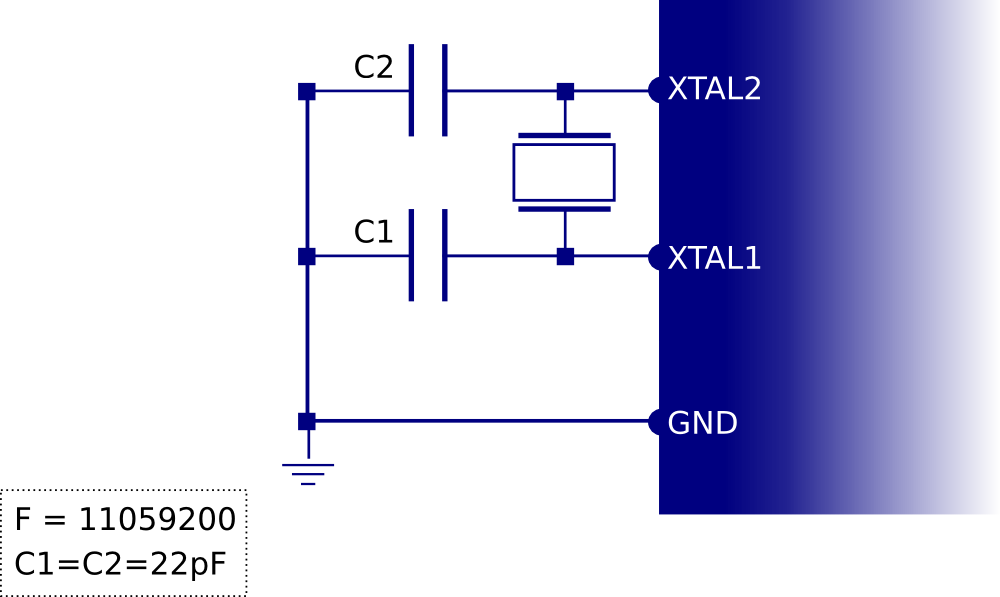
\includegraphics[width=300pt]{./images/esq_osc.png}
\caption{Esquema de conexión del oscilador externo.}
\label{fig:esq_osc}
\end{figure}

\subsubsection{Recepción}

Como el microcontrolador dispone de un periférico específico para la implementación de comunicaciones serie que permite el modo de trabajo asíncrono con dos contactos asociados en el empaquetado, siempre y cuando la señales sean TTL compatibles, no es necesaria la adición de ningún componente externo.

Tal como se ha descrito en la sección \ref{subsec:trans_fis}, las señales provenientes del ordenador se adecuan mediante el circuito integrado MAX232\cite{max232} a niveles apropiados. Simplemente se debe conectar la salida adecuada (en este caso R2OUT, el contacto 9 del integrado) a la entrada asociada en el microcontrolador, el contacto 2 (RXD).

\subsubsection{Muestra}
\label{subsubsec:muestra}

Una matriz de LEDs no es más que una serie de LEDs dispuestos de forma matricial y garantizando que todos aquellos situados en una fila tengan un contacto en común (en el diseño desarrollado, el ánodo), y aquellos situados en una columna el otro (el cátodo). La diferencia de tensión adecuada entre el ánodo (número de fila) y el cátodo (número de columna), encenderá el LED apropiado. Gestionando la tensión en todas las filas y todas las columnas se puede controlar qué LEDs se encienden y cuáles se mantienen apagados.

\begin{figure}[!htp]
\centering
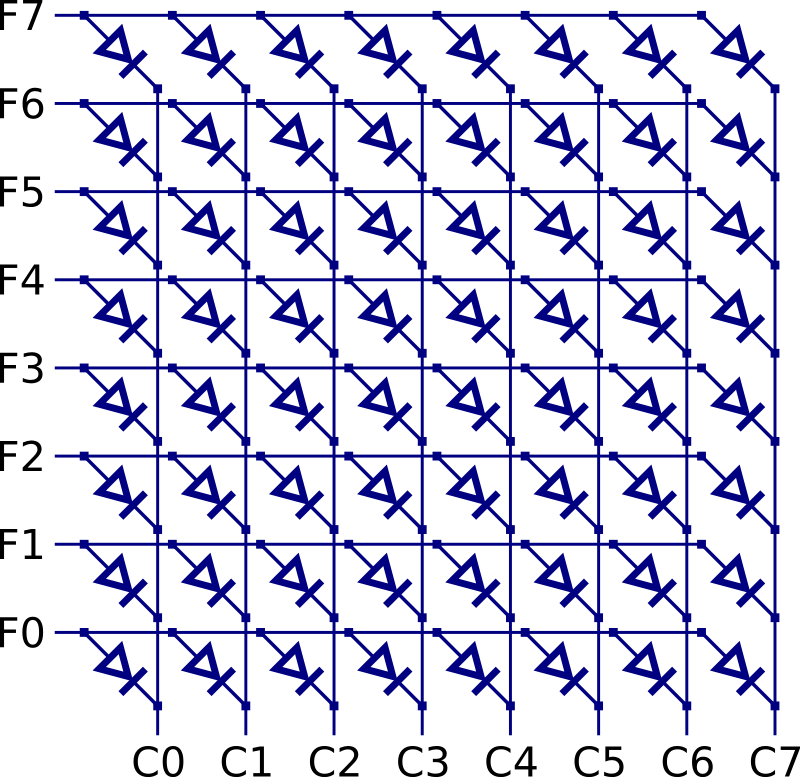
\includegraphics[width=200pt]{./images/esq_matriz.png}
\caption{Esquema de conexión de una matriz de LEDs 8x8.}
\label{fig:esq_matriz}
\end{figure}

La matriz puede fabricarse mediante la correcta colocación y conexionado de LEDs discretos, tal como ilustra la figura \ref{fig:esq_matriz}. Sin embargo, el número de contactos a conectar resulta lo bastante elevado como para resultar una labor tediosa: para una matriz de 8x8 se deben conectar 8x8x2=128 contactos. Existen en el mercado matrices ya empaquetadas con sólo el número de contactos correspondiente al número de filas y el número de columnas. Para una matriz de 8x8 se tendrían 8+8=16 contactos. La comodidad y el ahorro tanto en complejidad como en tiempo sin duda obligan a valorar muy positivamente esta posibilidad.

Para el desarrollo del prototipo de este proyecto, se ha utilizado un modelo comercial de 8x8\cite{matrix} del tipo columna-ánodo/fila-cátodo, debido a que era el modelo más accesible. Sin embargo, dado que la lógica se había considerado para una arquitectura donde las filas estuvieran conectadas a los ánodos, se ha optado por conectar los contactos descritos en la hoja de características como de columna a las filas, y viceversa.

La solución más rápida para gestionar una matriz de 8x8 mediante el microcontrolador consistiría en conectar cada uno de los contactos de ésta a un contacto del microcontrolador. Esto no resulta un problema para una matriz del tamaño descrito, pues disponemos de más 16 de contactos en el microcontrolador. Sin embargo, el objetivo de este proyecto es poder escalar el número de columnas para poder controlar carteles del tamaño deseado. Si se quisieran controlar 30 columnas, serían necesarios 38 contactos, de los cuales no se dispone. Es por esta razón por la que se ha optado por controlar la matriz de forma dinámica, haciendo uso de la multiplexación de las filas y utilizando registros de desplazamiento\cite{shiftr}.

Aprovechando que el microcontrolador funciona a una velocidad mucho mayor que la que el ojo humano es capaz de apreciar, se activarán las filas una por una, en lugar de encender todas ellas al mismo tiempo. Suponiendo que se trabaja con ocho filas, cada una de ellas estará encendida 1/8 parte del ciclo total de actualización. Como el ciclo total será menor que el tiempo mínimo apreciable, la sensación será la de estar viendo todas las filas iluminadas al mismo tiempo. Asumiendo que cada fila se encenderá por separado y nunca habrá dos de ellas activas al mismo tiempo, los LEDs que se encenderán vendrán determinados por el valor que tengan los contactos de las columnas en el momento de activación de una fila concreta. Ahí es donde cumplen su función los registros de desplazamiento: almacenarán los datos de las columnas durante el tiempo en que ésta esté activa. La comunicación entre el microcontrolador y un registro de desplazamiento es serie síncrona. Como es unidireccional, sólo necesitamos dos contactos, el de dato y el de reloj (que serán controlados por el microcontrolador), además de la masa.

De entre los registros de desplazamiento disponibles en el mercado, se ha optado por el 74HC164 \cite{164} en empaquetado PDIP de 14 contactos. Se trata de un modelo con dos contactos de entrada serie (1:A y 2:B), a las cuales se les realiza una operación lógica AND, y salida en paralelo de ocho bits. Puesto que no se necesitan las dos líneas de datos, se han conectado ambas entradas entre sí y al contacto de salida que se ha escogido en el microcontrolador para esta función (15:PB1). Las ocho salidas se han conectado a las respectivas columnas por medio de sendas resistencias \footnote{La función de las resistencias es limitar la tensión que caerá en los LEDs. El valor de éstas dependerá de la fuente con que se alimenten, como se verá al analizar la conexión de las filas.}, tal como describe la tabla \ref{tab:reg_col}.

\begin{table}[!htp]
\centering
\begin{tabular}[c]{|c|c|c|}
\hline
\multicolumn{2}{|c|}{\textbf{47HC164}} & \textbf{Matriz} \\
\hline
Q0 & 3 & C0 \\ \hline
Q1 & 4 & C1 \\ \hline
Q2 & 5 & C2 \\ \hline
Q3 & 6 & C3 \\ \hline
Q4 & 10 & C4 \\ \hline
Q5 & 11 & C5 \\ \hline
Q6 & 12 & C6 \\ \hline
Q7 & 13 & C7 \\
\hline
\end{tabular}
\caption{Conexiones entre el registro de desplazamiento y la matriz de LEDs.}
\label{tab:reg_col}
\end{table}

Los contactos de alimentación (14:VCC y 7:GND) se han conectado directamente a la fuente de alimentación. El reset global (9:$\overline{MR}$) se ha deshabilitado permanentemente dejándolo conectado a Vcc (el borrado se realizará por software al ejecutar la rutina de inicialización). El último contacto disponible, el de la señal de reloj (8:CP) se ha conectado al contacto escogido en el microcontrolador para dicha función (16:PB2).

Las salidas del microcontrolador pueden dar corriente suficiente para alimentar un reducido número de LEDs. Sin embargo, resulta claramente insuficiente a lo hora de trabajar con carteles de treinta, cuarenta o cincuenta columnas. En estos casos se debe utilizar un driver intermedio que actúe como etapa de potencia. Aunque el cartel del prototipo tiene pocas columnas, y a pesar de que en esas condiciones el microcontrolador podría alimentar los LEDs directamente, siempre es recomendable poner un driver para proteger el integrado de posible errores de montaje.

\begin{table}[!htp]
\centering
\begin{tabular}[c]{|c|c|c|}
\hline
\multicolumn{2}{|c|}{\textbf{Atmega48}} & \textbf{Matriz} \\
\hline
PC0 & 23 & F0 \\ \hline
PC1 & 24 & F1 \\ \hline
PC2 & 25 & F2 \\ \hline
PC3 & 26 & F3 \\ \hline
PC4 & 27 & F4 \\ \hline
PC5 & 28 & F5 \\ \hline
PD2 & 4  & F6 \\ \hline
PD3 & 5  & F7 \\
\hline
\end{tabular}
\caption{Conexiones entre el microcontrolador y la matriz de LEDs.}
\label{tab:filas}
\end{table}

En este proyecto las salidas del microcontrolador que deberán llevar driver son aquellas conectadas a las filas de la matriz de LEDs. Para conseguir la ganancia de potencia, se han utilizado transistores bipolares PNP\cite{140} que soportan una corriente de emisor de hasta 1.5A, lo cual permite conectar entre 75 y 100 columnas (en función de la corriente que consuman los LEDs). Al ser de tipo PNP, los transistores conducirán cuando la tensión en su base sea cero. Se debe tener en cuenta este hecho a la hora de realizar la programación de las rutinas del microcontrolador. Para desactivar una fila, por lo tanto, debería haber una tensión positiva en la base, lo cual se conseguirá activando la salida adecuada. Como sólo hace falta una pequeña corriente, se ha puesto una resistencia de 1K5 entre la salida y la base. El emisor de todos los transistores está conectado a la tensión de alimentación, mientras los colectores se conectan a las filas correspondientes de la matriz, de acuerdo con lo establecido por la tabla \ref{tab:filas}.

\begin{figure}[!htp]
\centering
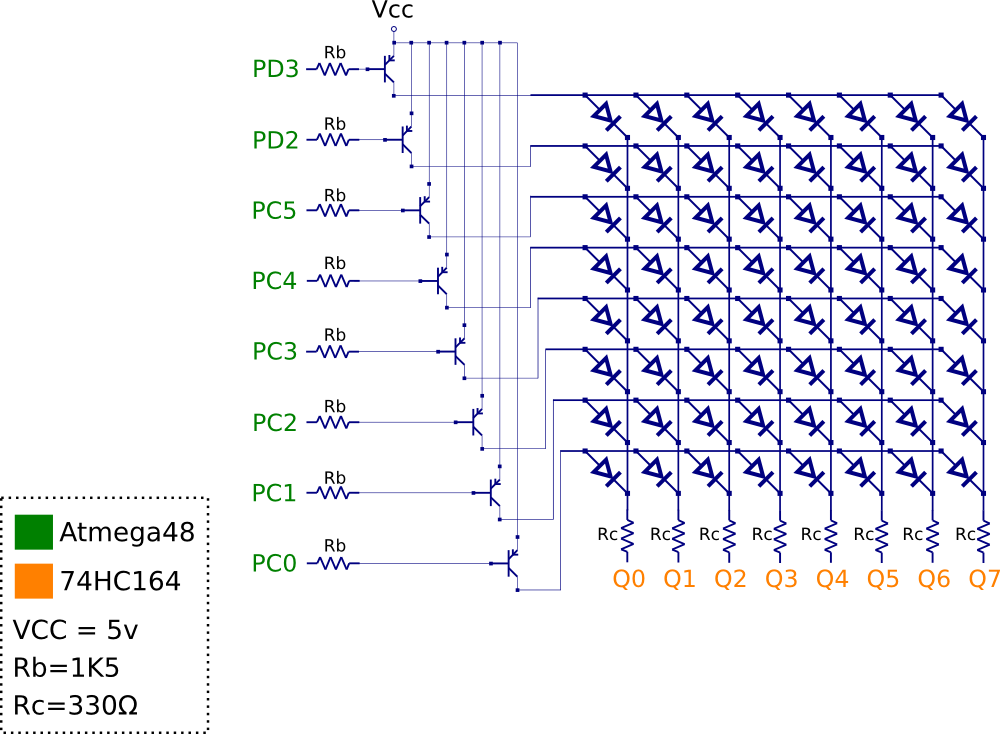
\includegraphics[width=350pt]{./images/esq_pnp.png}
\caption[Esquema de conexión matriz, microcontrolador y registro]{Esquema de conexión de la matriz al microcontrolador y al registro de desplazamiento.}
\label{fig:esq_pnp}
\end{figure}

Con la arquitectura descrita, cuando un transistor determinado conduzca y al menos una de las salidas del registro de desplazamiento esté a nivel bajo, habrá un LED que encuentre cero voltios (masa) en su cátodo y la tensión de alimentación en su ánodo. Lo más probable es que en estas condiciones el LED se queme, pues la alimentación será de aproximadamente cinco voltios. Para evitar que esto suceda, se podría sustituir la tensión en los emisores por una menor. Esto requiere dimensionar un divisor/reductor de tensión para soportar la corriente de todos los transistores. Desde un punto de vista práctico, resulta más fácil mantener ese mismo valor da alimentación e introducir resistencias entre los cátodos y las salidas del registro de desplazamiento, tal como ilustra la figura \ref{fig:esq_pnp}. Para el prototipo se han utilizado resistencias de 330$\Omega$.
